\mysubsubsection{FAQs and Onboarding Documentation}
Around 50\% of our projects have no actual FAQ or onboarding document, so there may exist opportunities to help newcomers by creating additional content. Only 8\% have an initial contact designated. That may be due to varying org structures, possibly even reflecting a deliberate choice to have the entry point be distributed and/or in flux (according to needs). Both the contact people and the dispatch of inquiries may be handled on ad hoc voluntary bases. Since members probably do have forum identities or other contact points, presumably, newbies can take initiative and contact them.

\begin{figure}[ht!]
\centering
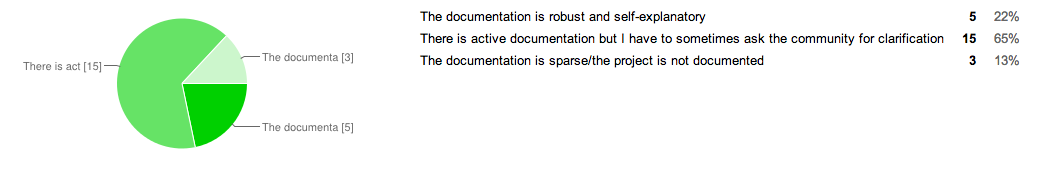
\includegraphics[width=120mm]{chapters/img/documentation.png}
\caption{How well are projects documented }
\label{overflow}
\end{figure}

Onboarding practice documentation may exhibit the potential for qualitative analysis, such as text analysis. (Perhaps just raising the issue itself would to project leads would raise interesting questions about governance and organizational processes). There might be correlations between FAQ/onboarding info available and the org structure/governance of the actual projects.(Of course, the product and/or nature of the project is also relevant). A summary follows of the projects and the types of onboarding guidance they provide, which often indicate the types of newcomer that may be targeted:

Hypothesis: Development-centric (may be sufficient for their needs)
Peerlibrary: Severeal different ways to contribute are listed and described. Since a member of our own group wrote it, it may not be a coincidence that this is one of the best all-purpose joining guides.
Mozilla PDF: Mentions that all ideas are open (also, was mainly bug, feature, and development-oriented)
Courtlistener: Has a great "ways to help" page
Facebook React: Developer and bug-centric, but also apologizes that they are still working on improving transparency and making a smoother, easier flow for contributors.
Chromium: Developer-centric
Civi-CRM: no FAQ, but does express and embrace a  "just dive in" culture, which may be sufficient
Geonode: The "about us" page is a bit FAQ-like, with some info on getting started, contact info, etc.
OaklandWiki(a site of the Localwiki project): it's a wiki which requires no login to contribute content. One can immediatley add or edit content with no account. There is no apparent moderation, so they may someday have problems with quality or spam.
Mifos: Complex options, but anyone can create an account. The ways to contribute are mainly technical, and some contribution screens require login, but many volunteering can be found in their volunteer sections-- the site was a bit fragmented. Some confusion may arise from the availability of both "contributor" and "volunteer" sections and subsections. The technical and non-technical areas had various options and areas. Presumably more options to participate become available after creating a free account for login access.

OTHER PROJECTS: The other projects do not yet have any FAQ or onboarding documentation.

Since there may be shared responsibilty, or unclear responsibility, in various organizations for marketing and community-building (these functions may be absorbed by members in decentralized fashion), it is sometimes not clear whether improving onboarding information would benefit the projects, or decisions have already been made that the current practices are sufficient. There was a striking variety of information available to help people with various backgrounds and skill levels join the communities. 




